\documentclass[a4paper,oneside,12pt]{extreport}

\usepackage{mmap}
\usepackage[T2A]{fontenc}
\usepackage[utf8]{inputenc}
\usepackage[english,russian]{babel}


% Текст отчёта следует печатать, соблюдая следующие размеры полей:
% левое — 30 мм, правое — 15 мм, верхнее и нижнее — 20 мм.
\usepackage[left=20mm, right=15mm, top=15mm, bottom=15mm]{geometry}

% \setlength{\parindent}{1.25cm} % Абзацный отступ

\usepackage{setspace}
%\onehalfspacing % Полуторный интервал

\frenchspacing % Равномерные пробелы
\usepackage{indentfirst} % Красная строка

\usepackage{microtype}
\sloppy

\usepackage{titlesec}
\titlespacing*{\chapter}{0pt}{-30pt}{8pt}
\titlespacing*{\section}{\parindent}{*4}{*4}
\titlespacing*{\subsection}{\parindent}{*4}{*4}
\titleformat{\chapter}{\LARGE\bfseries}{\thechapter}{20pt}{\LARGE\bfseries}
\titleformat{\section}{\Large\bfseries}{\thesection}{40pt}{\Large\bfseries}

\usepackage{graphicx}
\usepackage{caption}

\usepackage[unicode,pdftex]{hyperref}
\hypersetup{hidelinks}

%% title begin
\usepackage{wrapfig}

\makeatletter
	\def\vhrulefill#1{\leavevmode\leaders\hrule\@height#1\hfill \kern\z@}
\makeatother
%% title end

%% begin code
\usepackage{listings}
\usepackage{xcolor}

\lstset{
	basicstyle=\footnotesize\ttfamily,
	breakatwhitespace=true,
	breaklines=true,
	commentstyle=\color{gray},
	frame=single,
	keywordstyle=\color{blue},
	stringstyle=\color{red},
	tabsize=8
}

\lstdefinestyle{lispinline}{
	frame=none,
	language=Lisp
}

\newcommand{\code}[1]{\texttt{#1}}
%% end code

%% begin theorem
\usepackage{amsthm}

\makeatletter
\newtheoremstyle{indented}
	{}% measure of space to leave above the theorem
	{}% measure of space to leave below the theorem
	{}% name of font to use in the body of the theorem
	{\parindent}% measure of space to indent
	{\bfseries}% name of head font
	{.}% punctuation between head and body
	{ }% space after theorem head; " " = normal interword space
	{}% header specification (empty for default)
\makeatother

\theoremstyle{indented}

\newtheorem{definition}{Определение}[section]
\newtheorem{example}{Пример}[section]
\newtheorem{theorem}{Теорема}[section]
\newtheorem{task}{Задание}

\makeatletter
\DeclareRobustCommand\bfseriesitshape{%
	\not@math@alphabet\itshapebfseries\relax
	\fontseries\bfdefault
	\fontshape\itdefault
	\selectfont
}
\makeatother

\DeclareTextFontCommand{\textbfit}{\bfseriesitshape}
\DeclareTextFontCommand{\define}{\bfseriesitshape}
%% end theorem

%% begin columns
\usepackage{etoolbox,refcount}
\usepackage{multicol}

\newcounter{countitems}
\newcounter{nextitemizecount}
\newcommand{\setupcountitems}{%
	\stepcounter{nextitemizecount}%
	\setcounter{countitems}{0}%
	\preto\item{\stepcounter{countitems}}%
}
\makeatletter
\newcommand{\computecountitems}{%
	\edef\@currentlabel{\number\c@countitems}%
	\label{countitems@\number\numexpr\value{nextitemizecount}-1\relax}%
}
\newcommand{\nextitemizecount}{%
	\getrefnumber{countitems@\number\c@nextitemizecount}%
}
\newcommand{\previtemizecount}{%
	\getrefnumber{countitems@\number\numexpr\value{nextitemizecount}-1\relax}%
}
\makeatother
\newenvironment{AutoMultiColItemize}{%
	\ifnumcomp{\nextitemizecount}{>}{3}{\begin{multicols}{2}}{}%
		\setupcountitems\begin{itemize}}%
		{\end{itemize}%
		\unskip\computecountitems\ifnumcomp{\previtemizecount}{>}{3}{\end{multicols}}{}}
\makeatother
\newenvironment{AutoMultiColEnumerate}{%
	\ifnumcomp{\nextitemizecount}{>}{3}{\begin{multicols}{2}}{}%
		\setupcountitems\begin{enumerate}}%
		{\end{enumerate}%
		\unskip\computecountitems\ifnumcomp{\previtemizecount}{>}{3}{\end{multicols}}{}}
%% end columns



\begin{document}

\begin{titlepage}
	\noindent\begin{minipage}{0.05\textwidth}
		
\includegraphics[scale=0.3]{inc/bmstu.png}
	\end{minipage}
	\hfill
	\begin{minipage}{0.85\textwidth}\raggedleft
		\begin{center}
			\fontsize{12pt}{0.3\baselineskip}\selectfont \textbf{Министерство науки и высшего образования Российской Федерации \\ Федеральное государственное бюджетное образовательное учреждение \\ высшего образования \\ <<Московский государственный технический университет \\ имени Н.Э. Баумана \\ (национальный исследовательский университет)>> \\ (МГТУ им. Н.Э. Баумана)}
		\end{center}
	\end{minipage}

	\begin{center}
		\fontsize{12pt}{0.1\baselineskip}\selectfont
		\noindent\makebox[\linewidth]{\rule{\textwidth}{4pt}} \makebox[\linewidth]{\rule{\textwidth}{1pt}}
	\end{center}

	\begin{flushleft}
		\fontsize{12pt}{0.8\baselineskip}\selectfont 
		
		ФАКУЛЬТЕТ \uline{<<\textbf{Информатика и системы управления}>> \hfill}

		КАФЕДРА \uline{\mbox{\hspace{4mm}} <<\textbf{Программное обеспечение ЭВМ и информационные технологии}>> \hfill}
	\end{flushleft}

	\vfill

	\begin{center}
		\fontsize{20pt}{\baselineskip}\selectfont

		\uline{\textbf{ОТЧЁТ ПО ПРОИЗВОДСТВЕННОЙ ПРАКТИКЕ}}
	\end{center}
	
	\vfill
	
	\begin{flushleft}
		\fontsize{12pt}{0.7\baselineskip}\selectfont

		Студент \uline{\mbox{\hspace{44mm}} Богаченко Артём Евгеньевич \hfill}
		
		Группа \uline{\mbox{\hspace{64mm}} ИУ7-65Б \hfill}
		
		Тип практики \uline{\mbox{\hspace{44mm}} Производственная \hfill}
		
		Название предприятия \uline{\mbox{\hspace{26mm}} ООО~<<Эррайвал РУС>> \hfill}
	\end{flushleft}	

	\vfill

	\begin{table}[h!]
		\fontsize{12pt}{0.7\baselineskip}\selectfont

		\begin{signstabular}[0.55]{p{7.25cm} >{\centering\arraybackslash}p{4cm} >{\centering\arraybackslash}p{4cm}}
		Студент & \uline{\mbox{\hspace*{4cm}}} & \uline{\hfill \textbf{Богаченко А. Е.} \hfill} \\
		& \scriptsize \textit{подпись, дата} & \scriptsize \textit{фамилия, и.о.}
		\end{signstabular}
	
		\vspace{\baselineskip}

		\begin{signstabular}[0.55]{p{7.25cm} >{\centering\arraybackslash}p{4cm} >{\centering\arraybackslash}p{4cm}}
			Руководитель практики & \uline{\mbox{\hspace*{4cm}}} & \uline{\hfill \textbf{Толпинская Н. Б.} \hfill} \\
			\mbox{\hspace*{1cm}} \scriptsize (от университета) & \scriptsize \textit{подпись, дата} & \scriptsize \textit{фамилия, и.о.}
		\end{signstabular}

		\vspace{\baselineskip}
		
		\begin{signstabular}[0.55]{p{7.25cm} >{\centering\arraybackslash}p{4cm} >{\centering\arraybackslash}p{4cm}}
			Руководитель практики & \uline{\mbox{\hspace*{4cm}}} & \uline{\hfill \textbf{Холодная Т. Ю.} \hfill} \\
			\mbox{\hspace*{1cm}} \scriptsize (от предприятия) & \scriptsize \textit{подпись, дата} & \scriptsize \textit{фамилия, и.о.}
		\end{signstabular}
	
		\vspace{\baselineskip}
		
		\begin{signstabular}[0.55]{p{7.25cm} >{\centering\arraybackslash}p{4cm} >{\centering\arraybackslash}p{4cm}}
			Оценка~~\uline{\hfill}
		\end{signstabular} 
	 
	\end{table}

	\vfill

	\begin{center}
		\normalsize \textit{\the\year~г.}
	\end{center}
\end{titlepage}

\section*{Теоретическая часть}

% \subsection*{Логическое программирование}

% \textbf{Логическое программирование} -- это программирование на знаниях. 
% Логическое программирование принципиально работает не с данными, а со знаниями.
% % В отличии от императивных яп (в них определяется порядком записи правил (команд) 
% Порядок действий в системе логического программирования prolog определяется алгоритмом унификации. 

% Программируя на императивным я.п., программист должен задать порядок действий,
% (который в дальнейшем будет последовательно выполнен), т.е. объяснить компьютеру \textbf{как} решать задачу.
% В случае декларативного я.п. программист должен описать \textbf{что} нужно решить (А уже с помощью алгоритма унификации будет решена задача)

% \subsection*{Элементы языка}

% \textbf{Элементы языка}: терм.

% \textbf{Терм} - это:
% \begin{enumerate}
%     \item \textbf{константа}:
%     \begin{enumerate}
%         \item число (пример: 1; 55; 12.32);
%         \item символьный атом. Начинается со  \textbf{строчной} буквы и используется для обозначения конкретного объекта предметной области или для обозначения конкретного отношения (пример: alice, iu7\_63B);
%         \item строка - последовательность символов, заключенная в кавычки (пример: "Элис Сукочева").
%     \end{enumerate}
%     \item \textbf{переменная}
%     \begin{enumerate}
%         \item Именнованная - комбинация символов, цифр и '\_', которая начинается с \textbf{прописной} буквы или с символа '\_' (пример: Name, \_A). Переменные могут связываться с различными объектами – конкретизироваться;
%         \item Анонимная - обозначается символом '\_'. Анонимные переменные не могут быть связаны со значением.
%     \end{enumerate}
%     \item \textbf{составной терм} - взаимосвязанная информация. Показывает связь между объектами. Т.е. кто от чего зависит. 
%     Синтаксис: \textbf{$f(t_1, t_2, ... , t_m)$}, где $f$ - функтор - символьная константа, обозначающая имя отношения. $t_1$, $t_2$, ... , $t_m$ - термы, являющиеся аргументами. Арность - число аргументов. (Пример: учится(элис, мгту) - знание о то, что Элис учится в МГТУ.
% \end{enumerate}


\subsection*{Программа на prolog}

\textbf{Программа на prolog} - база знаний и вопрос. 

База знаний - это факты и правила. Каждое предложение (факт или правило) должно заканчиваться точкой.

\textbf{Правило} имеет вид:
    A :- $B_1$, ... , $B_n$
    
A - заголовок правила (терм).

$B_1$, ... , $B_n$ - тело правила (термы). 

Символ ":-" это специальный символ-разделитель.

\textbf{Факт} – это частный случай правила. Факт – это предложение, в котором отсутствует тело
(т.е. тело пустое). 
% В фактах присутствую только заголовки, а значит знания в заголовках.

\textbf{Заголовок} - составной терм, который содержит знание. Знания в заголовках.

\textbf{В теле} прописаны условия истинности этого знания (которое написано в заголовке).

В разделе \textbf{CLAUSES} записываются факты и правила.

Пример:

\begin{lstlisting}[language=Prolog]
CLAUSES
    study(alice, bmstu).
    study(ivan, bmstu).
\end{lstlisting}
    
% Вопрос - вид предложения.
\textbf{Вопрос} - частный случай правила, состоит только из тела (составного терма или нескольких составных термов).
Используется, чтобы определить, выполняется ли некоторое отношение между описанными в программе объектами.
Ответом может быть "Yes" или "No".

В разделе GOAL содержатся цели, которые нужно достигнуть. 
Главная задача заключается в том, чтобы дать ответ "Yes" на поставленный вопрос.
В случае, если система не может ответить "Yes", система отвечает "No".

Пример:
\begin{lstlisting}[language=Prolog]
GOAL
    study(alice, bmstu) % Yes
\end{lstlisting}

% Переменные предназначены для передачи значений "во времени и в пространстве".
% Конкретизация переменной - связь переменной с объектом.

\subsection*{Механизм унификации}
\textbf{Механизм унификации} (подбор нужного решения).
Поиск ответа на поставленный вопрос заключается в поиске нужного знания с помощью механизма унификации. Данный механизм встроен в систему и недоступен программисту.

\textbf{Процедуры} - совокупность правил, заголовки которых имеют одно и то же имя и одну и ту же арность.

\textbf{Предикат} - отношение, определяемое процедурой.

\newpage

\section*{Практическая часть л.р.14}

\begin{task}
    Используя базу знаний, хранящую знания (лаб. 13):
    \begin{enumerate}
        \item «Телефонный справочник»: Фамилия, Номер  тел, Адрес – структура (Город, Улица, Номер дома, Номер кв)
        \item «Автомобили»: Фамилия\_владельца, Марка, Цвет, Стоимость, и др.,
        \item «Вкладчики банков»: Фамилия, Банк, счет, сумма, др.
    \end{enumerate}
    Владелец может иметь несколько телефонов, автомобилей, вкладов (Факты).
    В разных городах есть однофамильцы, в одном городе – фамилия уникальна.

    Используя конъюнктивное правило и простой вопрос, обеспечить возможность
    поиска:

    По Марке и Цвету автомобиля найти Фамилию, Город, Телефон и Банки, в которых
    владелец автомобиля имеет вклады.
    Владельцев может быть несколько (не более 3-х), один и ни одного.
    \begin{lstlisting}[language=Prolog]
DOMAINS 
    surname = symbol.
    phone_number = symbol.
    address_struct = address(symbol, symbol, integer, integer).

    label = symbol.
    color = symbol.
    price = integer.
    
    bank = symbol.
    score = integer.
    sum = integer.

PREDICATES
    phonebook(surname, phone_number, address_struct).
    car(surname, label, color, price).
    bank_depositor(surname, bank, score, sum).
    
    f(label, color, surname, symbol, phone_number, bank).

CLAUSES
    phonebook("Tilov", "+100", address("Moscow", "2 baumanskaya", 57, 25)).
    phonebook("Alovik", "+111", address("Moscow", "3 baumanskaya", 50, 75)).
    
    car("Tilov", "Buick", "black", 12000000).
    car("Alovik", "Buick", "black", 1500000).
    car("Tilov", "Cadillac", "white", 22000000).
    
    bank_depositor("Alovik", "sberbank", 10000, 25000).
    bank_depositor("Tilov", "vtb", 21500, 3000).
    
    f(Label, Color, Surname, City, Phone, BankName) :- 
            car(Surname, Label, Color, _), 
            phonebook(Surname, Phone, address(City, _, _, _)),
            bank_depositor(Surname, BankName, _, _).
    
GOAL
    f("Buick", "black", SurnameR, CityR, PhoneR, BankNameR).       
    \end{lstlisting}
\end{task}

\newpage

\begin{task}
    Словесно подробно описать порядок формирования ответа (в виде таблицы).

    \begin{figure}[ht!]
    	\centering{
    		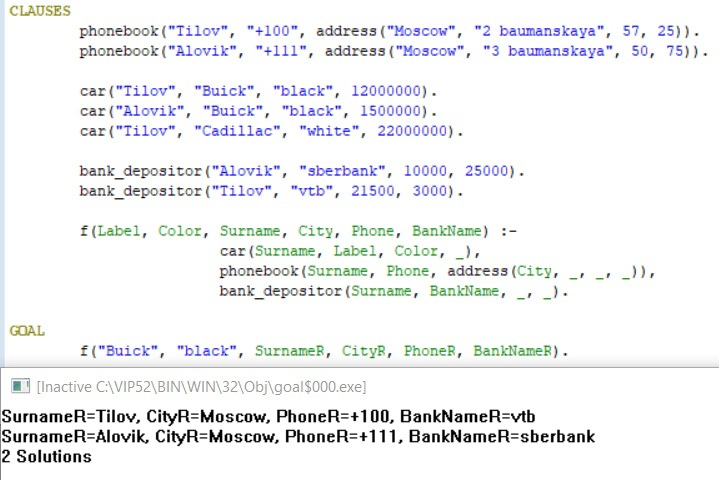
\includegraphics[width=0.9\textwidth]{img/res_lab_14/2.jpg}
    		\caption{Результат работы}
            \label{ref:fig5} }
    \end{figure}

%     % TODO: Делать от руки?

%     \begin{center}
%         \begin{tabular}{|c|c|}
%         \hline
%         Сравниваемые термы, результат, подстановка & Дальнейшие действия \\
%         \hline
%         f("Buick", "black", SurnameR, City, & Состояние резольвенты:\\ 
%         PhoneR, BankNameR) = & f("Buick", "black", SurnameR, City, \\ 
%         phonebook("Tilov", "+100", &  PhoneR, BankNameR) \\
%         address("Moscow", "2 baumanskaya", 57, 25)) &  \\
%         Не унифицируемы  &  \\
%         \hline
%         \end{tabular}
%     \end{center}
\end{task}

\newpage

\section*{Практическая часть л.р.15}

\begin{task}
    Создать базу знаний «Собственники» , дополнив базу знаний, хранящую знания
    \begin{enumerate}
        \item Телефонный справочник: Фамилия, Номер телефона, Адрес – структура (Город, Улица, номер дома, номер кв),
        \item Автомобили: Фамилия владельца, Марка, Цвет, Стоимость, и др.,
        \item Вкладчики банков: Фамилия, Банк, счет, сумма, др.
    Владелец может иметь несколько телефонов, автомобилей, вкладов (Факты).
    Используя правила, обеспечить возможность поиска:
    \end{enumerate}

    знаниями о дополнительной собственности владельца. Преобразовать знания об
    автомобиле к форме знаний о собственности.
    Вид собственности (кроме автомобиля):

    \begin{enumerate}
        \item строение, стоимость и другие его характеристики;
        \item участок, стоимость и другие его характеристики;
        \item водный\_транспорт, стоимость и другие его характеристики.
    \end{enumerate}

    Описать и использовать вариантный домен: Собственность.
    Владелец может иметь, но только один объект каждого вида собственности 
    (это касается и автомобиля), или не иметь некоторых видов собственности.
    Используя конъюнктивное правило и разные формы задания одного вопроса
    (пояснять для какого номер задания – какой вопрос), 
    обеспечить возможность поиска:

    \begin{enumerate}
        \item Названий всех объектов собственности заданного субъекта,
        \item Названий и стоимости всех объектов собственности заданного субъекта,
    \end{enumerate}

    \begin{lstlisting}[language=Prolog]
DOMAINS 
    surname = symbol.
    phone_number = symbol.
    address_struct = address(symbol, symbol, integer, integer).

    name = symbol.
    color = symbol.
    price = integer.
    size = integer.
    year_of_release = integer.
    
    bank = symbol.
    score = integer.
    sum = integer.
    
    property = 
        car(name, price, color, year_of_release);
        building(name, price, size);
        plane(name, price, size).

PREDICATES
    phonebook(surname, phone_number, address_struct).
    bank_depositor(surname, bank, score, sum).
    own(surname, property).
    
    propertyNames(surname, name).
    namesAndPrices(surname, name, price).

CLAUSES
    phonebook("Tilov", "+100", address("Moscow", "2 baumanskaya", 57, 25)).
    phonebook("Alovik", "+111", address("Moscow", "3 baumanskaya", 50, 75)).
    
    bank_depositor("Alovik", "sberbank", 10000, 25000).
    bank_depositor("Tilov", "vtb", 21500, 3000).

    own("Tilov", car("Buick", 1200, "black", 1993)).
    own("Tilov", plane("S7", 8500, 80)).
    
    own("Alovik", car("Lg", 21500, "red", 1900)).
    own("Alovik", building ("little House", 45000,  250)).
    own("Alovik", plane("NewAir", 9000, 95)).
    
    propertyNames(Surname, NameProperty) :- own(Surname, car(NameProperty, _, _, _)).
    propertyNames(Surname, NameProperty) :- own(Surname, building(NameProperty, _, _)).
    propertyNames(Surname, NameProperty) :- own(Surname, plane(NameProperty, _, _)).
        
    namesAndPrices(Surname, NameProperty, PriceProperty) :- own(Surname, car(NameProperty, PriceProperty, _, _)).
    namesAndPrices(Surname, NameProperty, PriceProperty) :- own(Surname, building(NameProperty, PriceProperty, _)).
    namesAndPrices(Surname, NameProperty, PriceProperty) :- own(Surname, plane(NameProperty, PriceProperty, _)).

GOAL
    propertyNames("Tilov", NamePropertyR).
    \end{lstlisting}

    \begin{figure}[ht!]
    	\centering{
    		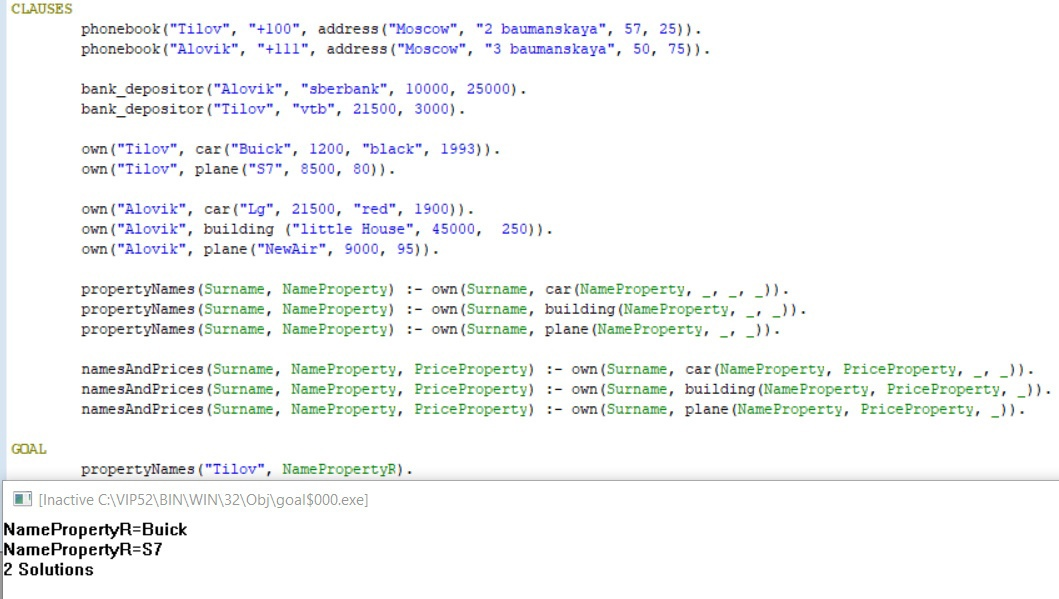
\includegraphics[width=0.9\textwidth]{img/res_lab_15/2.jpg}
    		\caption{Задание 1. Результат работы}}
    \end{figure}

    \begin{figure}[ht!]
    	\centering{
    		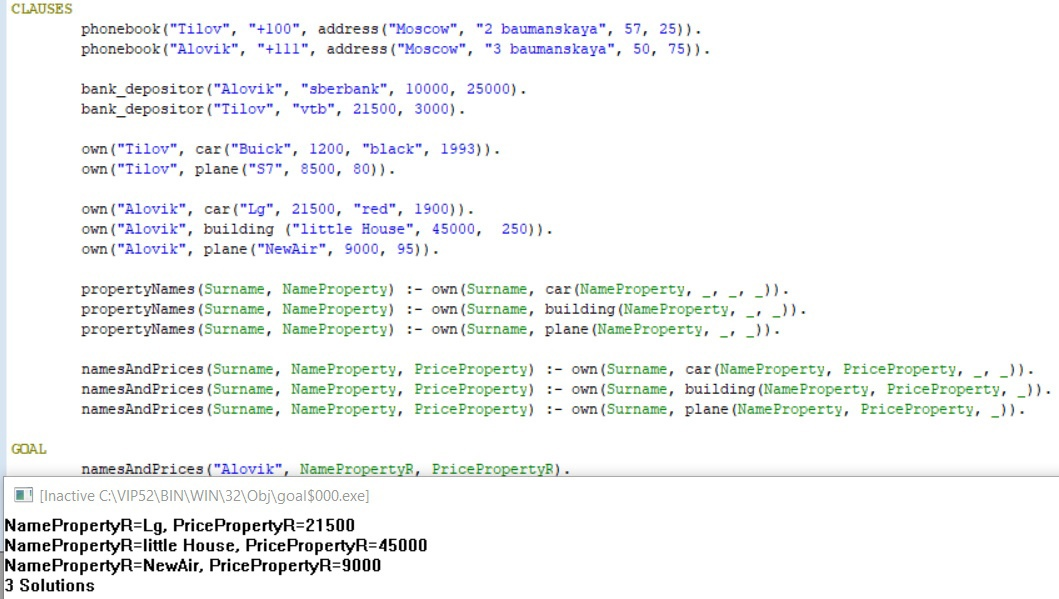
\includegraphics[width=0.9\textwidth]{img/res_lab_15/1.jpg}
    		\caption{Задание 2. Результат работы}}
    \end{figure}

\end{task}

\newpage

\begin{task}
    Иная формулировка.

    \begin{lstlisting}[language=Prolog]
DOMAINS 
    surname = symbol.
    phone_number = symbol.
    address_struct = address(symbol, symbol, integer, integer).

    name = symbol.
    color = symbol.
    price = integer.
    size = integer.
    year_of_release = integer.
    
    bank = symbol.
    score = integer.
    sum = integer.
    
    property = 
        car(price, color, year_of_release);
        building(price, size);
        plane(price, size).

PREDICATES
    phonebook(surname, phone_number, address_struct).
    bank_depositor(surname, bank, score, sum).
    own(surname, property).
    
    propertyNames(surname, name).
    namesAndPrices(surname, symbol, price).

CLAUSES
    phonebook("Tilov", "+100", address("Moscow", "2 baumanskaya", 57, 25)).
    phonebook("Alovik", "+111", address("Moscow", "3 baumanskaya", 50, 75)).
    
    bank_depositor("Alovik", "sberbank", 10000, 25000).
    bank_depositor("Tilov", "vtb", 21500, 3000).

    own("Tilov", car(1200, "black", 1993)).
    own("Tilov", plane(8500, 80)).
    
    own("Alovik", car(21500, "red", 1900)).
    own("Alovik", building (45000,  250)).
    own("Alovik", plane(9000, 95)).
    
    propertyNames(Surname, "car") :- own(Surname, car(_, _, _)).
    propertyNames(Surname, "building") :- own(Surname, building(_, _)).
    propertyNames(Surname, "plane") :- own(Surname, plane(_, _)).
        
    namesAndPrices(Surname, "car", PriceProperty) :- own(Surname, car(PriceProperty, _, _)).
    namesAndPrices(Surname, "building", PriceProperty) :- own(Surname, building(PriceProperty, _)).
    namesAndPrices(Surname, "plane", PriceProperty) :- own(Surname, plane(PriceProperty, _)).

GOAL
    %propertyNames("Tilov", NamePropertyR).
    namesAndPrices("Alovik", NamePropertyR, PricePropertyR).
    \end{lstlisting}

\end{task}

\begin{figure}[ht!]
    \centering{
        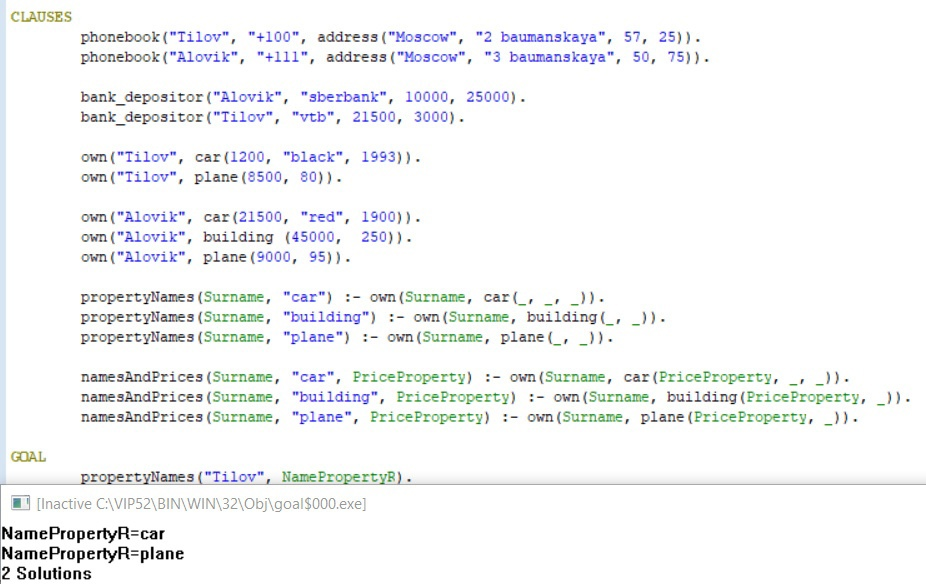
\includegraphics[width=0.9\textwidth]{img/res_lab_15/2_2.jpg}
        \caption{Задание 1. Результат работы}}
\end{figure}

\begin{figure}[ht!]
    \centering{
        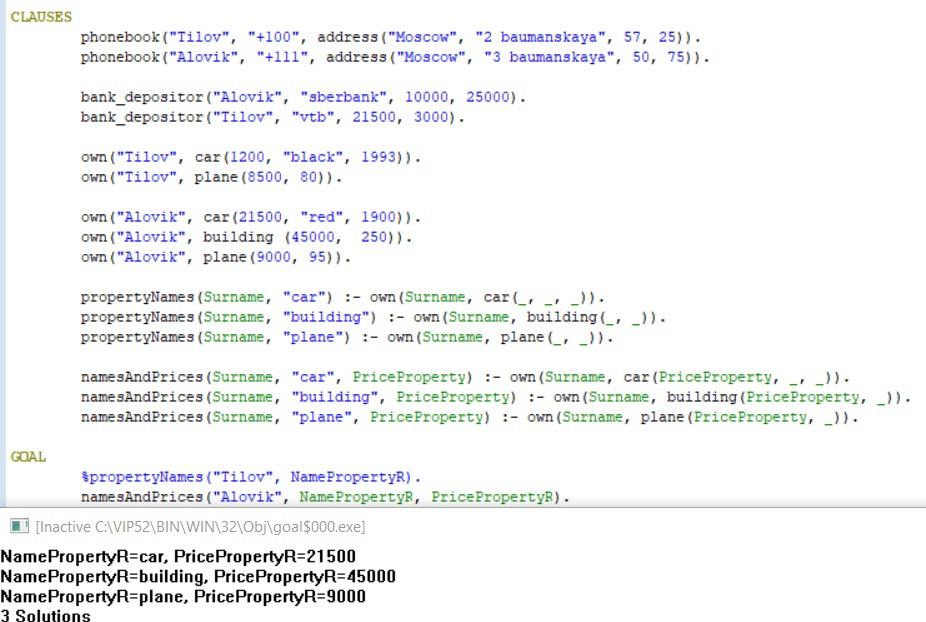
\includegraphics[width=0.9\textwidth]{img/res_lab_15/2_1.jpg}
        \caption{Задание 2. Результат работы}}
\end{figure}

\newpage


\end{document}